%
% lagrangekurve.tex -- 
%
% (c) 2024 Prof Dr Andreas Müller
%
\begin{figure}
\centering
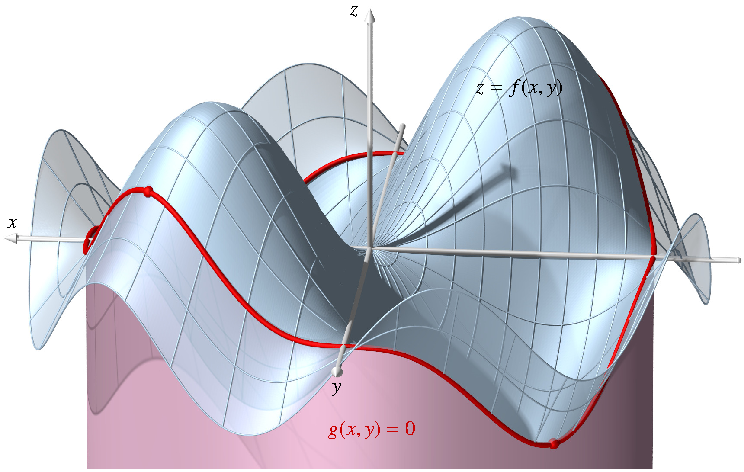
\includegraphics{chapters/010-fuvar/images/lagrangekurve.pdf}
\caption{Extremalproblem mit Nebenbedingung. 
Gesucht ist das Maximum der Funktion $f(x,y)$ unter der Nebenbedingunge
$g(x,y)=0$, dargestellt durch den roten Zylinder.
Gesucht sind die Extrema auf der roten Kurve, die Funktionswerte von 
$f(x,y)$ für Argumente darstellt, die die Nebenbedingung erfüllen.
\label{buch:fuvar:nebenbedingungen:fig:lagrangekurve}}
\end{figure}
